\documentclass{article} % Try also "scrartcl" or "paper"

\usepackage[utf8]{inputenc}
\usepackage[T1]{fontenc}
\usepackage[margin=1.5cm]{geometry}
\geometry{a4paper}
\usepackage{minted}
\usepackage[hyphens]{url}
\usepackage{graphicx}
\usepackage{float}

\newcommand{\codeJSinline}[2] {
	#1 : \mintinline{javascript}{#2} \linebreak
  }

\newcommand{\codeHTMLinline}[2] {
	#1 : \mintinline{HTML}{#2}
  }
  
\newcommand{\codeCSSinline}[2] {
	#1 : \mintinline{CSS}{#2} 
  }

\newenvironment{codeJS}[1]{%
#1 :  %
\minted{javascript}%  % use \minted and \endminted instead of \begin{} an \end{} to solve errors...
}{%
\endminted%
}

\newenvironment{codeHTML}[1]{%
#1 :  %
\minted{HTML}%  % use \minted and \endminted instead of \begin{} an \end{} to solve errors...
}{%
\endminted%
}

\newenvironment{codeCSS}[1]{%
#1 :  %
\minted{CSS}%  % use \minted and \endminted instead of \begin{} an \end{} to solve errors...
}{%
\endminted%
}

\title{Introduction au développement informatique}
\author{Matthieu Falce \& Jordan Bouchoucha}

\begin{document}
\maketitle

Le but de ce TP est de vous faire réaliser une page web interactive en 2h. 

Vous aller créer un mini-jeu dans lequel l'utilisateur va devoir retrouver un nombre choisi par l'ordinateur.

Cela vous permettra de découvrir le Javascript, HTML et CSS. Pour les points de syntaxes ou pour tous point de blocage, vous référez à la "feuille de triche", si ce n'est pas clair, n'hésitez pas à nous poser des questions.

\section{Javascript}

Le Javascript contient "l'intelligence" de votre jeu. Il va permettre au navigateur d'indiquer à l'utilisateur si le nombre donné est plus petit, plus grand ou si c'est le bon. 

\subsection{Implémenter l'algorithme}

Nous avons trouver l'algorithme a implémenter durant la présentation. 

\begin{center}
	\emph{\`A vous de l'implémenter. }
\end{center}

Notions à utiliser : les types de variables, les boucles, les conditions et tests ainsi que les fonctions \texttt{input}, \texttt{console.log}, \texttt{alert}.

\subsection{Mettre du code dans une fonction}

Pour pouvoir faciliter la suite, vous aller \texttt{encapsuler} la logique du jeu dans une fonction. Elle agira comme une boite noire qui fait ce qu'il faut. 

Pour un nombre donné en paramètre, la fonction va écrire si c'est plus, moins ou si c'est bon. 

N'hésitez pas à vous servir de ce que vous avez fait précédemment. 

\vspace{0.5cm}

\begin{minipage}[t]{0.45\linewidth}
	\begin{codeJS}{Squelette de la fonction}
	function tour(nombre){
		// ici c'est à vous	
		...
	}
	\end{codeJS}
\end{minipage} \hfill
\begin{minipage}[t]{0.45\linewidth}
	\begin{codeJS}{Contrat d'utilisation}
	// imaginons que le nombre 
	// à trouver soit 32
	tour(13); // écrit "c'est plus"
	tour(43); // écrit "c'est moins" 
	tour(32); // écrit "c'est bon"
	\end{codeJS}

\end{minipage}




\section{HTML}

Les sites n'utilisent plus de pop-up pour l'interaction depuis environs 25 ans. Construction une page web pour communiquer avec l'utilisateur.

\subsection{Construction de la page}

Réalisez une page ayant cette structure

\begin{minipage}[c]{0.45\linewidth}
\centering 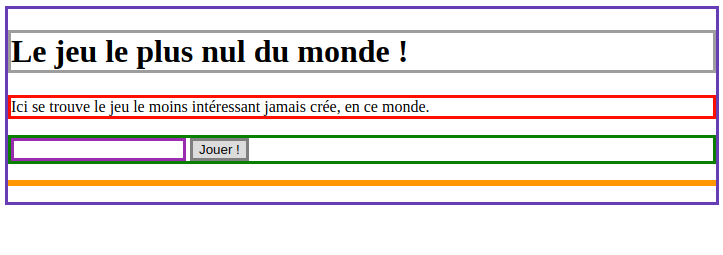
\includegraphics[width=1\linewidth]{html_structure.png}
\end{minipage} \hfill
\begin{minipage}[c]{0.45\linewidth}
\centering 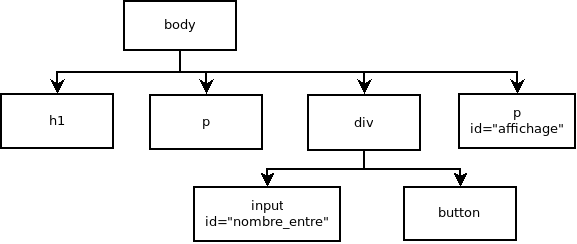
\includegraphics[width=1\linewidth]{html_arbre.png}
\end{minipage}


\subsection{Adapter le jeu à la programmation réactive}

Avant, nous avions une "boucle principale" pour continuer le jeu jusqu'à avoir trouver. A présent le navigateur nous en fourni une. Il faut légèrement changer le code de la fonction \texttt{tour} précédente. 

On peut faire en sorte que la validation du bouton lance un tour du jeu. Pour cela, nous allons faire une fonction \texttt{game} qui ne prend pas de paramètres. Nous allons dire au bouton de lancer la fonction lorsque l'on clique \codeJSinline{dessus}{<button onclick="game()" type="button">}

\begin{codeJS}{Structure de \texttt{game}}
	function game() {
		nombre_demande = get_input_number();
		tour(nombre_demande); // tour est la fonction précédente
	}

\end{codeJS}

\begin{codeJS}{Code supplémentaire fourni}
	function get_input_number(){
		// fonction permettant de récupérer le nombre dans le champs de texte
		return parseInt(document.getElementById('nombre_entre').value);
	}
\end{codeJS}


\subsection{Améliorer l'intéraction}

Un utilisateur n'a pas à regarder la console de son navigateur pour savoir s'il a le bon nombre ou pas... 

Utilisez le code suivant pour remplacer le \texttt{console.log} et mettre à jour des éléments de la page web.

\begin{codeJS}{Code supplémentaire fourni}
	function update_display(text){
		// fonction permettant de mettre à jour le paragraphe de résultat.
		document.getElementById('affichage').style.visibility = "visible";
		document.getElementById('affichage').textContent = text;
	}

	function update_background_color(color){
		// fonction permettant de mettre à jour la couleur de fond de la page.
		document.body.style.backgroundColor = color;
	}

\end{codeJS}

\section{CSS}

Cette page est moche. Améliorons là.

\subsection{Centrer les textes}

Utiliser \codeCSSinline{cette déclaration}{text-align: center;} pour centrer les textes sur une ligne. 

Où doit-on la placer pour tout centrer ?

\subsection{Couleurs}

Nous pouvons changer les couleurs du titre et du contenu. 

Que pensez-vous \codeCSSinline{de}{color: rgb(15, 15, 15);} \codeCSSinline{ou}{color: rgb(55, 55, 55);}

Nous pouvons également changer la couleur de fond de la page pour indiquer à l'utilisateur si c'est plus ou moins. Utiliser \texttt{update\_background\_color} défini précédemment pour le mettre à jour.

\section{Bonus}

\subsection{Si l'utilisateur ne rentre pas un nombre...}

Comment détecter si un utilisateur n'a pas entré un nombre ? Aller regarder la documentation des \texttt{NaN} pour voir comment les repérer.

\subsection{Centrer verticalement}

Le centrage vertical dans une page est (était...) un vrai problème en CSS. Regardez la documentation de flexbox pour avoir une solution actuelle.

\end{document}